\section{LITEX Solution}
\label{sec:solution}


As we have discussed in \S\ref{sec:problem}, a truly applicable off-chain
architecture needs to support the functionality of dynamical channel deposit and
withdrawl. Original Lightning Network assumes that the total funds in a channel
are throughout the channel's lifetime. Thus, there is no need to broadcast any
in-channel transactions.

\begin{figure}[H]
\centering
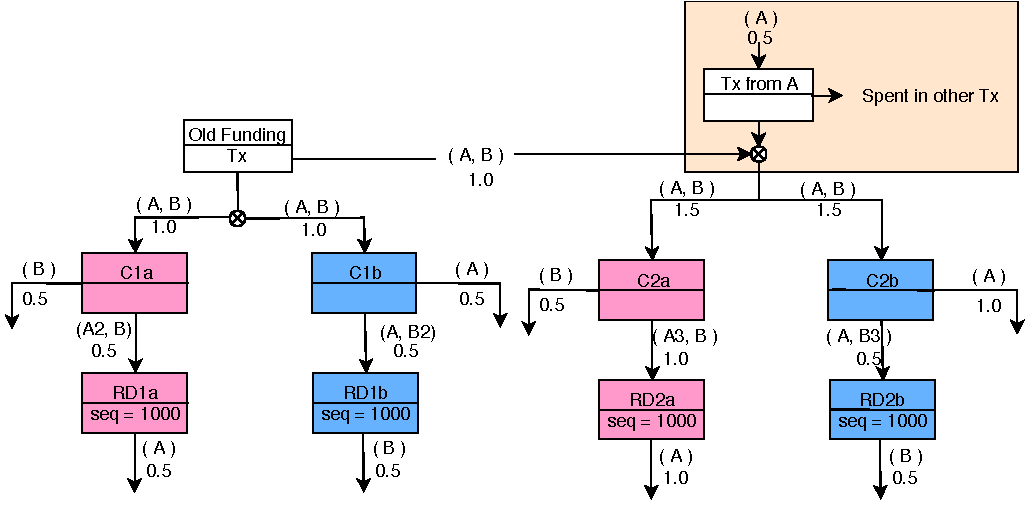
\includegraphics[width=4in]{figs/fake.pdf}
\vspace{-6pt}
\caption{If the deposit from Alice is not broadcasted, she may double spend it after agreement new Committment Transactions with Bob.}
\label{fig:fake}
\end{figure}

\begin{figure}[H]
\centering
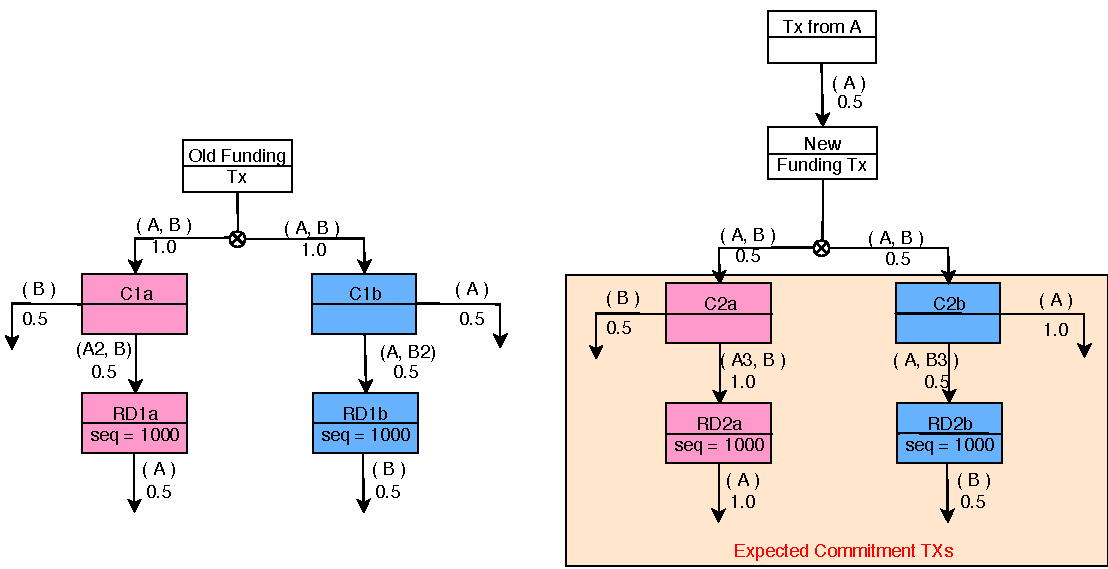
\includegraphics[width=4in]{figs/fund.pdf}
\vspace{-6pt}
\caption{A new Funding Transaction is constructed, the remaining problem is to connect it with old Funding Transaction(s).}
\label{fig:fund}
\end{figure}


When a deposit or a withdrawl occurs, the channel status is modified, which must be verified and recognized by most participants. Otherwise, the counterparty may claim a fake input and double-spend the fund. Figure~\ref{fig:fake} shows an example where Alice deposits 0.5 BTCs into the channel. The deposit results in an agreement on a pair of new Commitment Transactions with her counterparty Bob (1.0 BTC for Alice and 0.5 BTCs for Bob). If the deposit is not broadcast, Alice may spend the fund in other places. Although Bob can detect the double-spend by monitoring all on-chain transactions, he has no method to compensate himself.


Thus, it is necessary to broadcast any channel modification caused by deposit or
withdrawl. To broadcast the channel modification, a new funding transaction has to
be constructed. The channel deposit is shown in Figure~\ref{fig:fund}. In this case, the new Funding Transaction takes an UTXO from an external transaction for deposit. Therefore, broadcasting the funding transaction spends the UTXO so that it cannot be double-spent once the broadcast transaction is verified. The output of the new Funding Transaction is a pair of Commitment Transactions, each of which is held by the respective counterparty in the channel. In Figure~\ref{fig:fund}, the Commitment Transactions also rsult in RD2a and RD2 transactions, which prevent old Commitment Transactions from being broadcast.


The new funding transaction must interact with existing funding transactions to
ensure the validity of new Commitment Transactions. In particular, the total
amount of "vouts" must be equal to that of "vins." We also need to invalidate old Commitment Transactions, i.e., the counterparty who broadcasts any old commitment transaction will lose all his/her funds. Although broadcasting inevitably results in extra costs and delay, it is applicable because channel deposit and withdrawl do not occur frequently.


We now propose two separate approaches to support dynamic channel
deposit (i.e., splice-in) and withdrawl (i.e., splice-out). The two approaches are
differed by the layout of Funding Transactions, and we will elaborate both approaches as follows.

\begin{figure}[H]
\centering
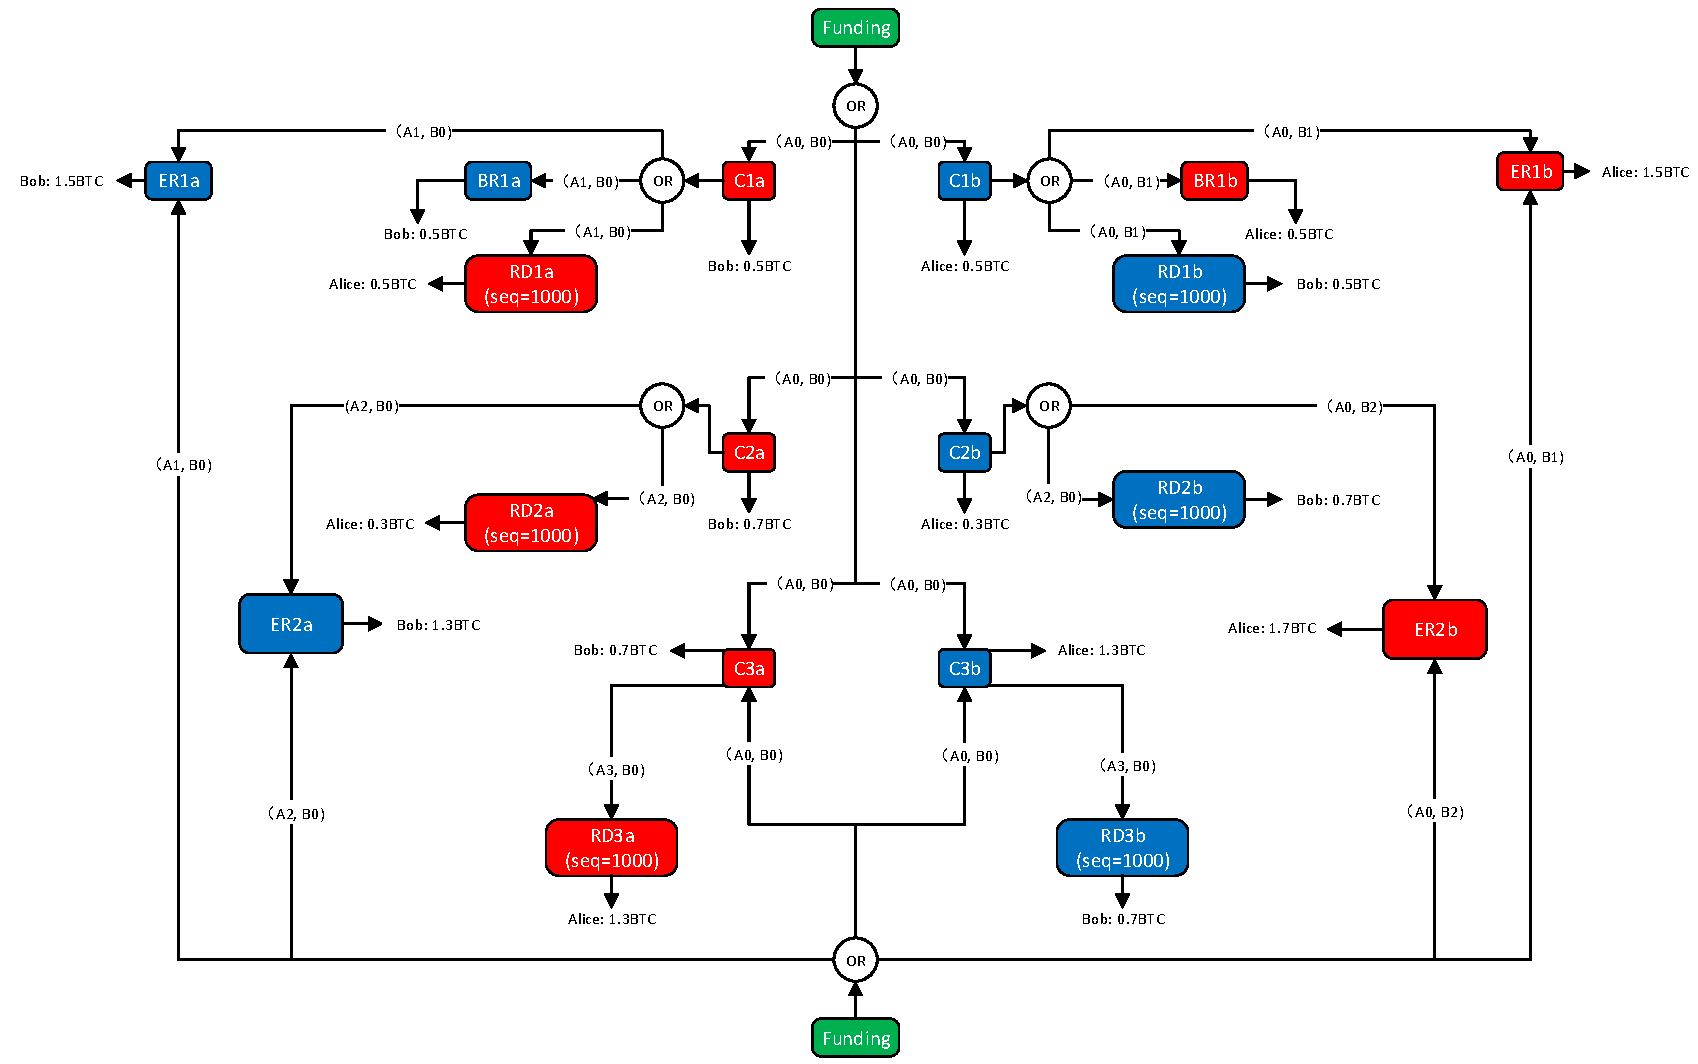
\includegraphics[width=6in]{figs/rsmc_new.pdf}
\vspace{-6pt}
\caption{FundPara RSMC transactions.}
\label{fig:rsmc_new}
\end{figure}

\begin{figure}[H]
\centering
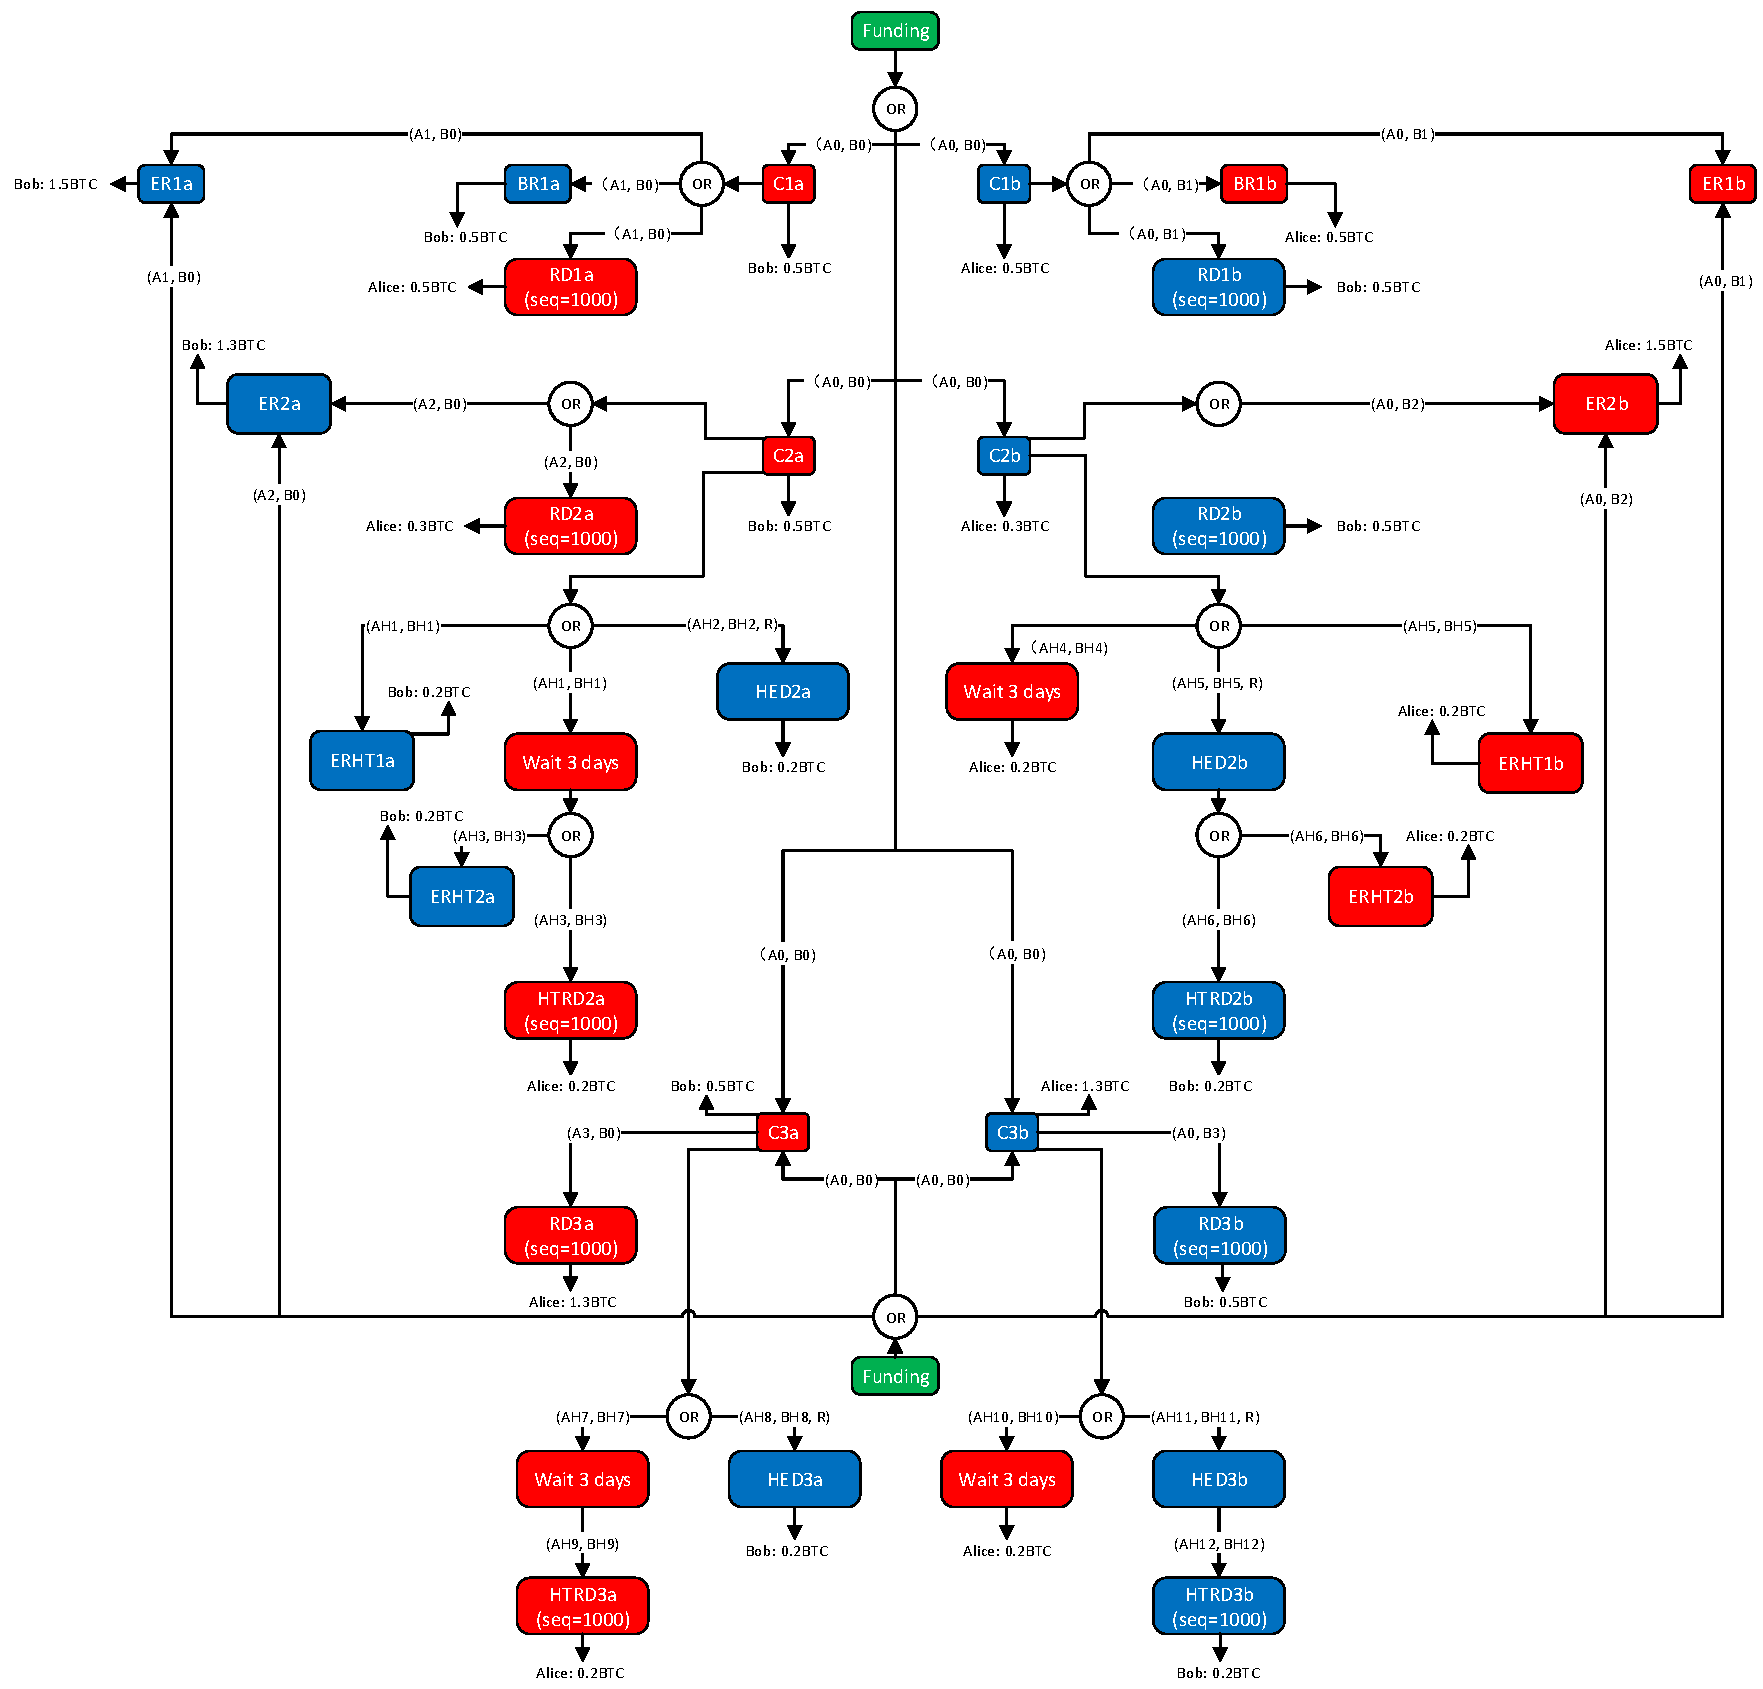
\includegraphics[width=6in]{figs/htlc_new.pdf}
\vspace{-6pt}
\caption{FundPara HTLC transactions.}
\label{fig:htlc_new}
\end{figure}

\subsection{FundPara}


The first approach {\em FundPara} enables each new commitment to take all Funding Transactions as its input. The benefit of this approach is that all Funding Transactions are parallel: counterparties can agree on new Commitment
Transactions with arbitrary combinations of Funding Transactions as input.
Figure~\ref{fig:rsmc_new} and~\ref{fig:htlc_new} show the details of channel
deposit for RSMC and HTLC. FundPara demands the invalidation of {\em all} existing Commitment Transactions, while RSMC also invalidates old commitment transactions by exchanging private keys. Thus, numerous keys are exchanged when a channel has made a large amount of transactions, resulting in poor scalability.

\begin{figure}[H]
\centering
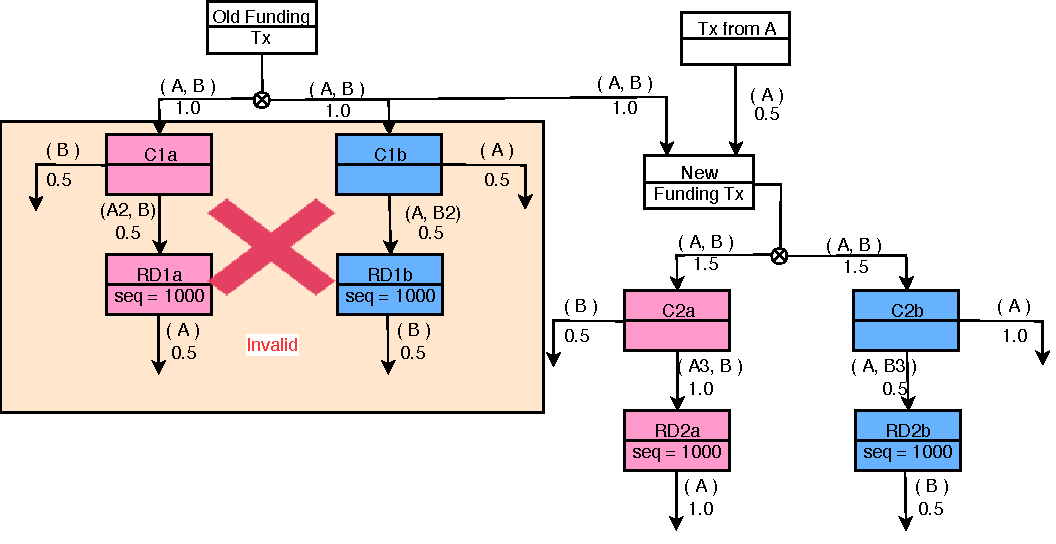
\includegraphics[width=4in]{figs/splice_in.pdf}
\vspace{-6pt}
\caption{FundCasc: Alice deposits 0.5 BTCs into the channel.}
\label{fig:splice_in}
\end{figure}

\subsection{FundCasc}


The second approach {\em FundCasc} cascades all funding transactions, i.e., the output UTXO of old Funding Transaction is directed as the "vin" of the new Funding
Transaction. Figure~\ref{fig:splice_in} depicts the solution. In Figure~\ref{fig:splice_in}, a new Funding Transaction takes two "vins:" one is the UTXO from the external transaction deposited by Alice, and the other is the UTXO from old Funding Transaction. Once the new Funding Transaction is verified on chain, all old Commitment Transactions that are derived from the old Funding Transaction become invalid. The reason is that all of them use the UTXO from old Funding Transaction as "vin", which has been spent by the new Funding Transaction. The new Funding Transaction has a "vout" with new funds in the channel. Then we use the "funding-vout" of the new Funding Transaction to create a pair of Commitment Transactions (C2a and C2b) for both participants of the channel.


Specifically, the splice-in proceeds as follows:
\begin{enumerate}
\item Creating a new Funding Transaction
\item Creating a pair of new Commitment Transactions (C2a and C2b), containing the corresponding RD2a and RD2b
\item Signing the new Commitment Transactions
\item Exchanging signatures for new Commitment Transactions
\item Signing a new Funding Transaction
\item Exchanging signatures for the new Funding Transaction
\item Broadcasting the new Funding Transaction
\end{enumerate}

\begin{figure}[H]
\centering
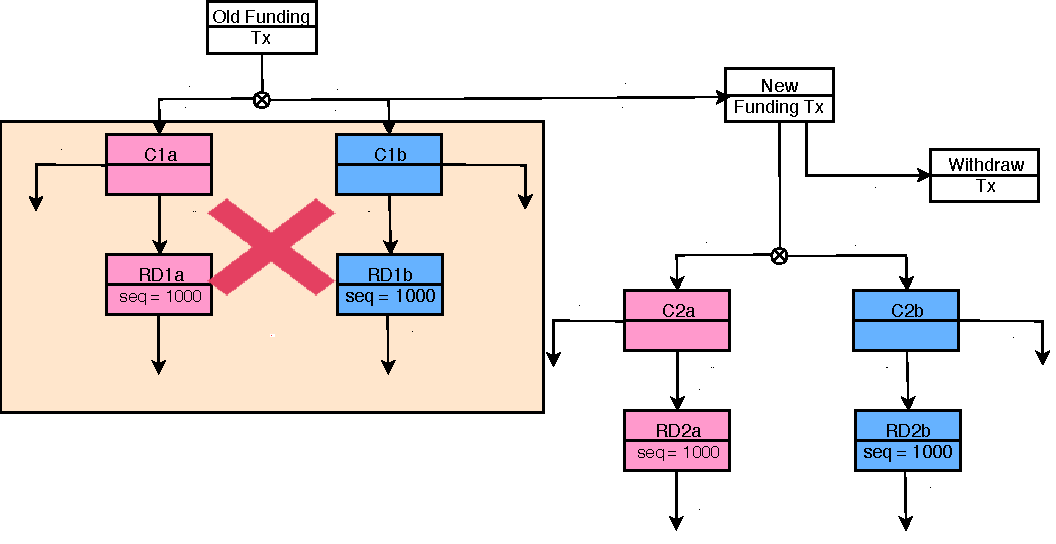
\includegraphics[width=4in]{figs/splice_out.pdf}
\vspace{-6pt}
\caption{FundCasc splice-out: Alice withdraws 0.4 BTCs from the channel.}
\label{fig:splice_out}
\end{figure}

\para{Splice-out.}
The solution of splice-out is similar to that of splice-in. Figure~\ref{fig:splice_out} shows the procedure. We construct a new Funding Transaction which takes the UTXO of an old Funding Transaction (1.0 BTC) as its only "vin". It produces two "vouts": one specifing the remaining fundings in the channel (0.6 BTCs), and the
other "vout" indicating the amount of funding withdrawn (0.4 BTCs). The remaining
fundings result in two Commitment Transactions, which corresponds to the fundings of both counterparties within the channel (0.1 BTCs for Alice and 0.5 BTCs for Bob).

\begin{figure}[H]
\centering
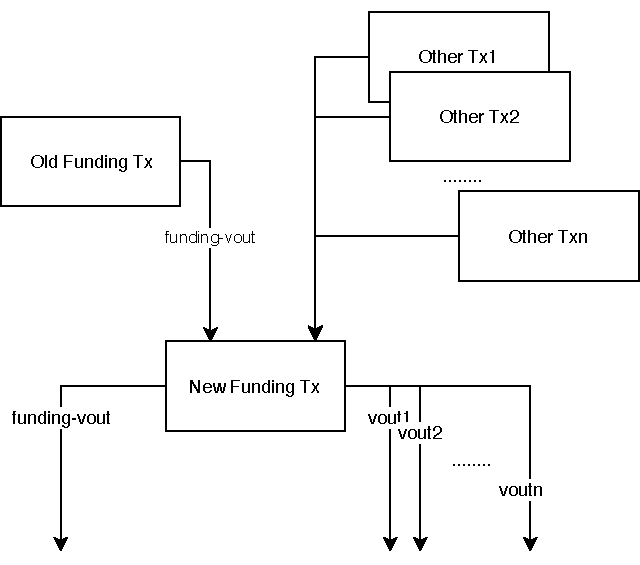
\includegraphics[width=3in]{figs/channel_change.pdf}
\vspace{-6pt}
\caption{LITEX general channel change: multiple "vins" and "vouts."}
\label{fig:change}
\end{figure}

\para{Extensions.}
The splice-in and splice-out of FundCasc have exactly one "vout" or "vin". In general, we can construct arbitrary number of "vins" and "vouts" for the new Funding Transaction whenever deemed necessary. Figure~\ref{fig:change} demonstrates a case with $n+1$ "vins" (one from previous Funding Transaction) and $n+1$ "vouts" (one from the channel).


This design brings great flexibility for channel management. For example,
Alice wants to deposit a large amount of funding into the channel but she only
has multiple small UTXO. At the same time, Bob intends to withdraw some fundings
to his various accounts. In this case, they can agree on a new Funding Transaction with multiple "vins" and "vouts".


The proposed approach is also compatible with previous approaches such as
channel rebalancing. For example, a participant can use the Circle Pay approach
to rebalance his/her fundings across multiple channel. When Circle Pay fails,
he/she may employ our proposed splice-in/splice-out approaches.
